\NeedsTeXFormat{LaTeX2e}
\documentclass[12pt,oneside,a4paper]{article}
\usepackage[left=2cm, right=2cm, top=1cm, bottom=2cm]{geometry}
\usepackage{amsmath,amsfonts,amssymb,amsthm}
\usepackage[utf8]{vietnam}
\usepackage{graphicx}
\usepackage[american]{circuitikz}
\usepackage{float}
\usepackage{mathptmx}
\usepackage{multicol}
\usepackage{enumitem} 
\usepackage{tasks} 
\usepackage{booktabs}
\usepackage{array}
\usepackage{caption}
\usepackage{hyperref}
\usepackage{pgfplots}

\everymath{\displaystyle}
\theoremstyle{definition}
\newtheorem{bt}{} 
\renewcommand{\thebt}{\textbf{\large Q\arabic{bt}}} 

\newcommand{\bb}[1]{\mathbb{#1}}

\newlist{questions}{enumerate}{1}
\setlist[questions]{label=\textbf{Q$_{\mathbf{\arabic*}}$:}, leftmargin=4em}

\settasks{label=\textbf{\Alph*.}, label-width=1.5em, item-indent=7mm}
\pgfplotsset{compat=1.18}

\begin{document}
	\renewcommand{\figurename}{Figure}
	\renewcommand{\tablename}{Table}
	
	\begin{center}
		\textbf{\Large EXPERIMENT 2}
		
		\vspace{0.5cm}
		\textbf{{\Large MEASUREMENT OF MAGNETIC FIELD INSIDE A}}
		
		\vspace{0.1cm}
		\textbf{{\Large SOLENOID WITH FINITE LENGTH}}
	\end{center}
	
	\vspace{0.5cm}
	
	\noindent
	\begin{minipage}[t]{0.5\textwidth}
		\vspace{0.5cm}
		\textbf{Class: IT-E10 02} \\[0.2cm]
		\textbf{Group: 3} \\[0.2cm]
		\textbf{Name: Nguyễn Trọng Phúc Anh} \\[0.2cm]
		\textbf{Student ID: 202516522}
	\end{minipage}%
	\begin{minipage}[t]{0.5\textwidth}
		\vspace{0pt}
		\centering
		\textit{\textbf{Verification of the instructors}} \\[0.2cm]
		\begin{tabular}{|p{3.5cm}|p{3.5cm}|}
			\hline
			& \\[2.5cm]
			\hline
		\end{tabular}
	\end{minipage}
	
	\vspace{0.8cm}
	
	\section*{1. DEVICES AND PURPOSE OF THE EXPERIMENT}
	\begin{center}
		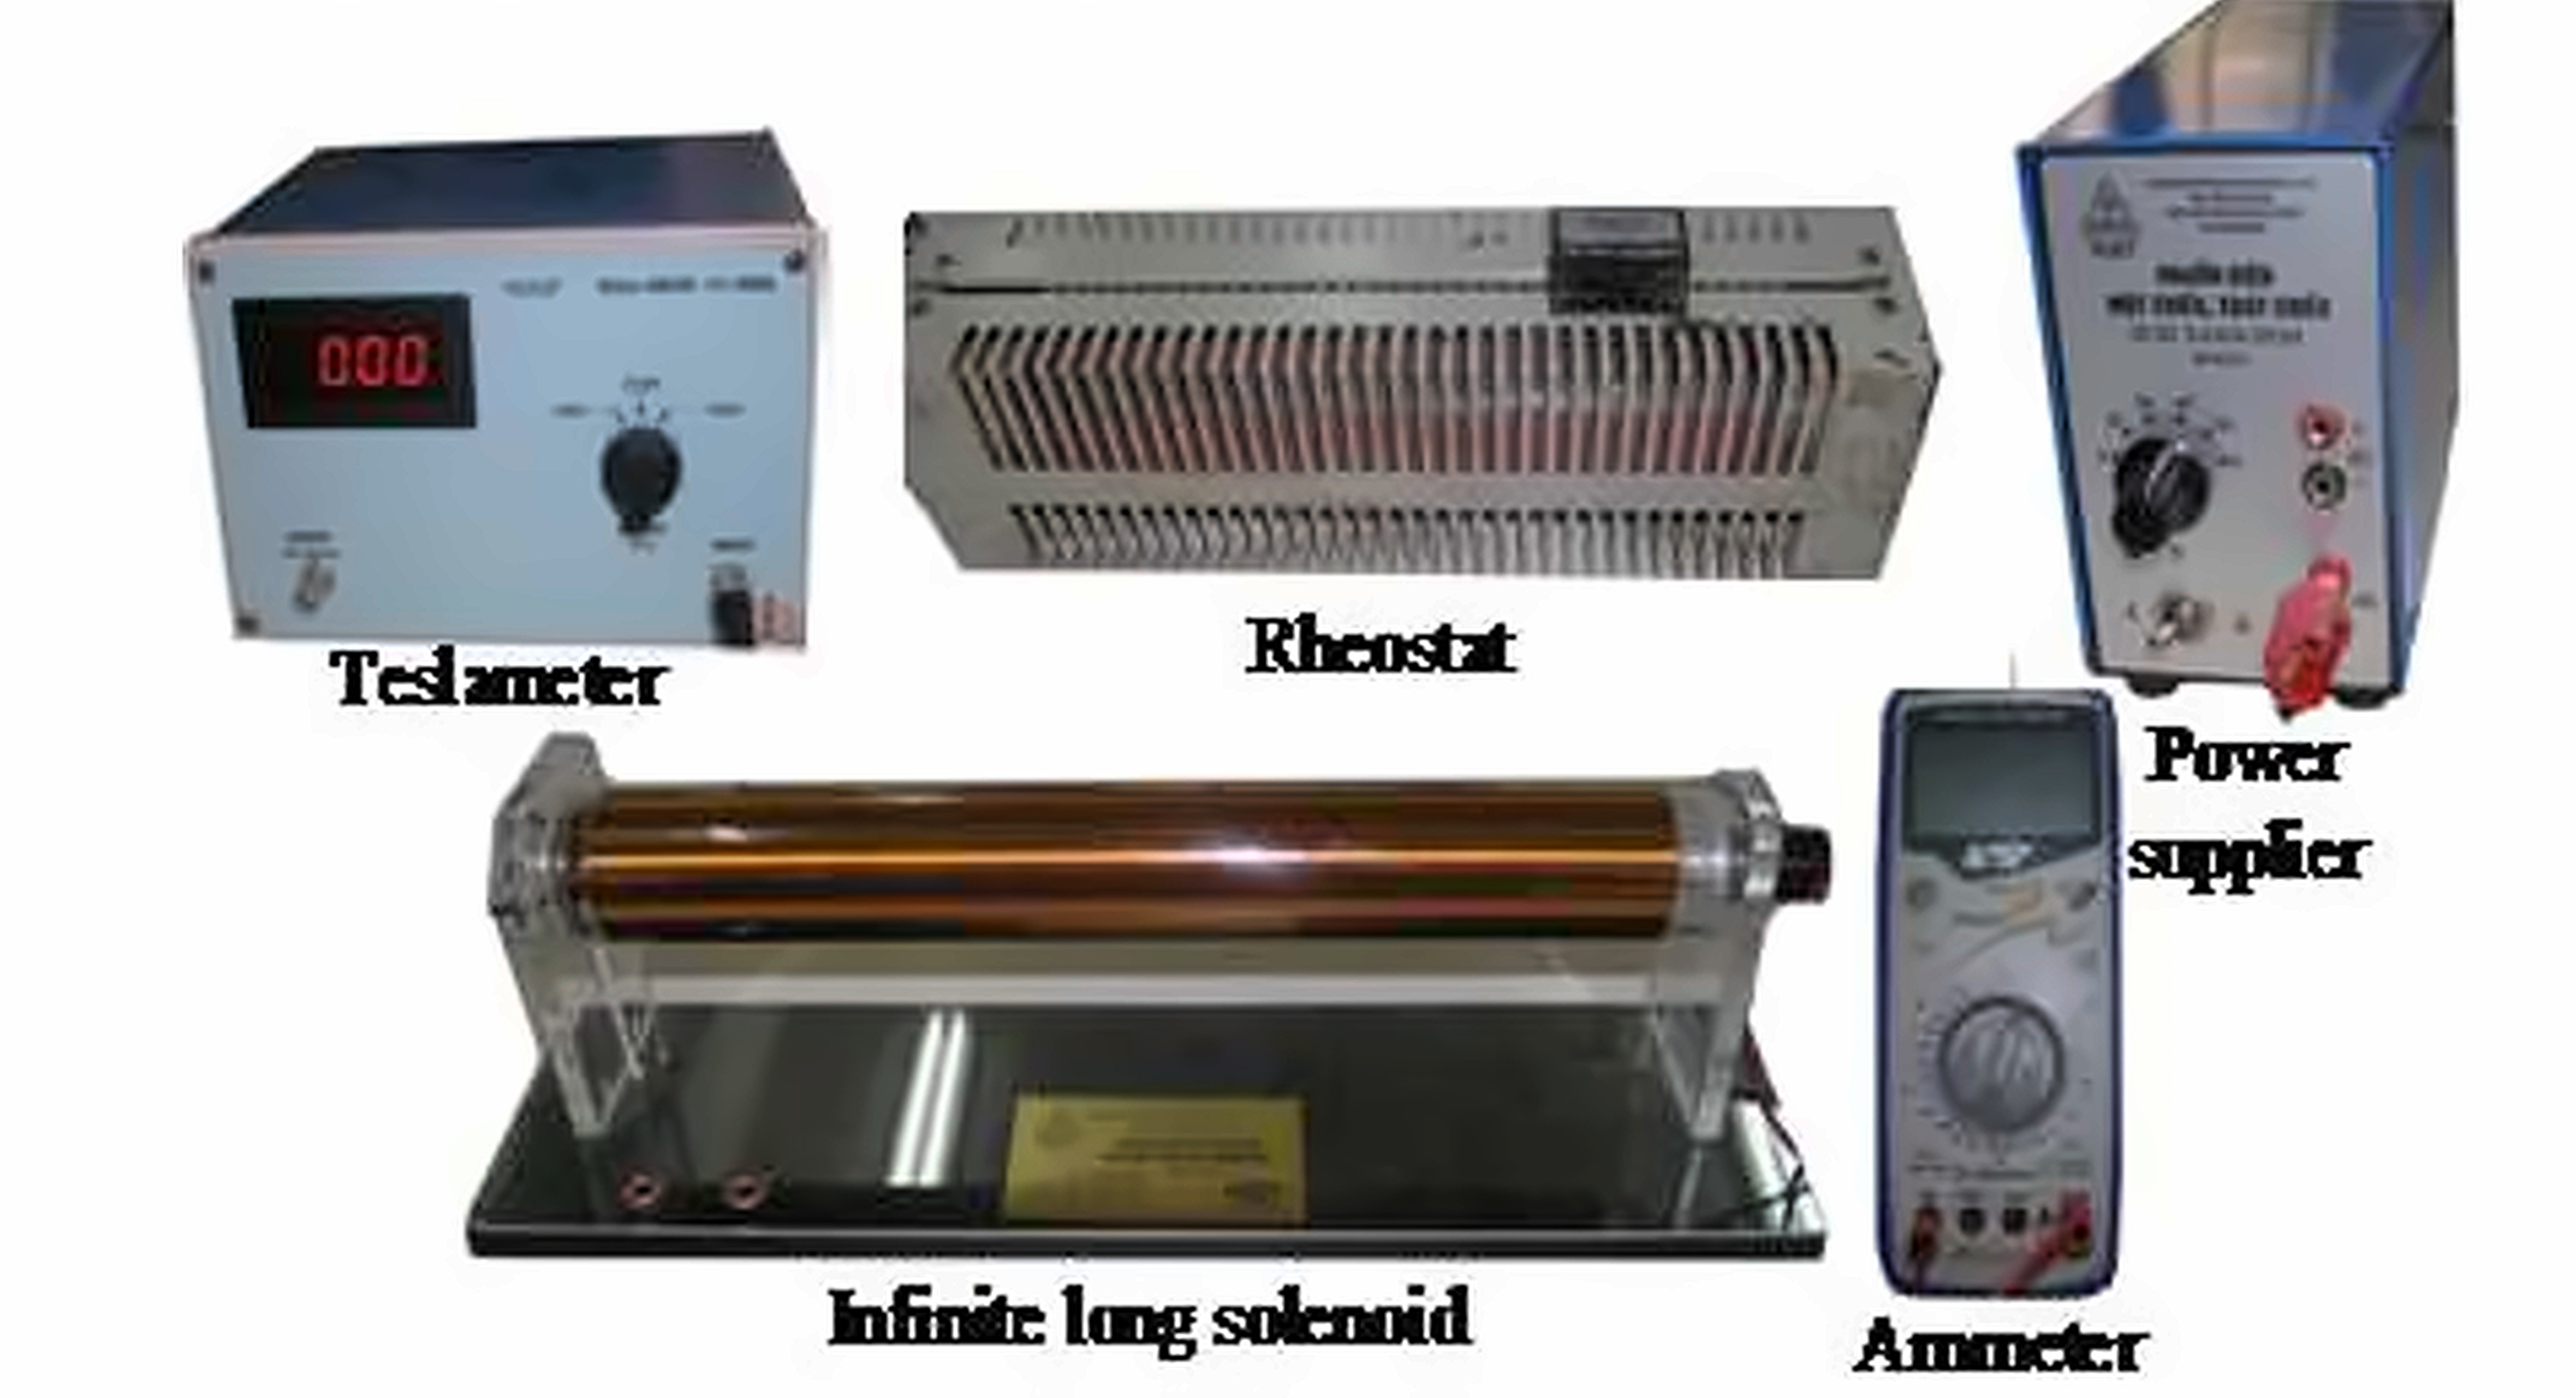
\includegraphics[width=0.75\textwidth]{Devices2 (2)}
	\end{center}
	\noindent
	The experiment is to study the magnetic field in a real solenoid and compare the obtained 
	results with the theoretical ones based on Biot-Savart’s law.
	
	
	\section*{2. THEORETICAL BACKGROUND}
	
	\noindent
	According to the Biot--Savart--Laplace law, the magnetic field $\vec{B}$ produced on the axis of a current-carrying loop is determined as follows:
	\begin{equation}
		B = \frac{\mu_0\mu_r}{4\pi}\displaystyle \int\limits_{0}^{2\pi R}\frac{I \sin\gamma \, dl}{r^2} = \frac{\mu_0\mu_r}{4\pi}\displaystyle \int\limits_{0}^{2\pi R}\frac{IR}{r^3} \, dl = \frac{\mu_0\mu_r}{2}\frac{IR^2}{r^3}
	\end{equation}
	\begin{center}
		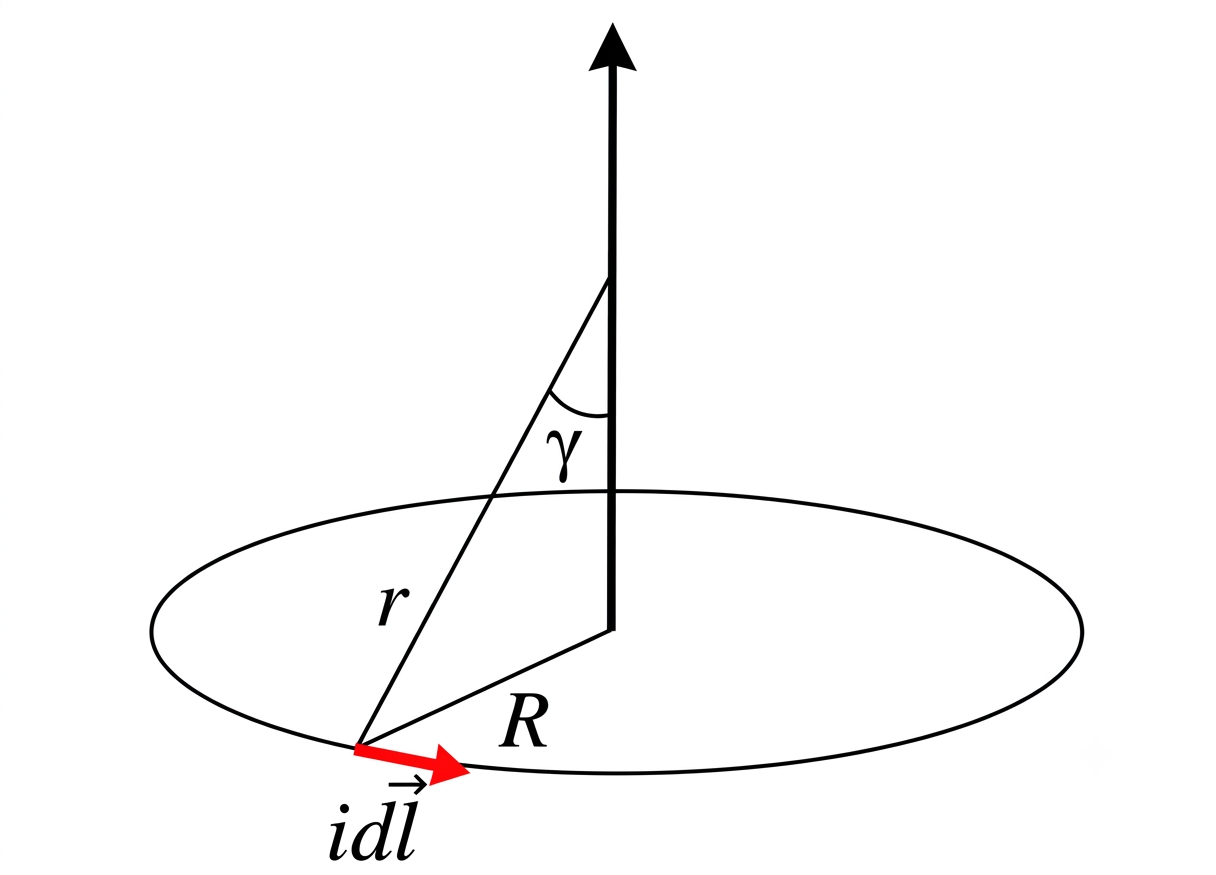
\includegraphics[width=0.4\textwidth]{Fig1}
		\captionof{figure}{\textit{ Magnetic field produced on the axis of a current-carrying coil. }}
	\end{center}
	
	\noindent
	A solenoid consists of a helical winding of wire on a cylinder, usually circular in cross section. There can be hundreds or thousands of closely spaced turns, each of which can be regarded as a circular loop (Fig.2a). Inside solenoid, the field lines are considered to be uniformly spaced as 
	shown in Fig.2b.
	\begin{center}
		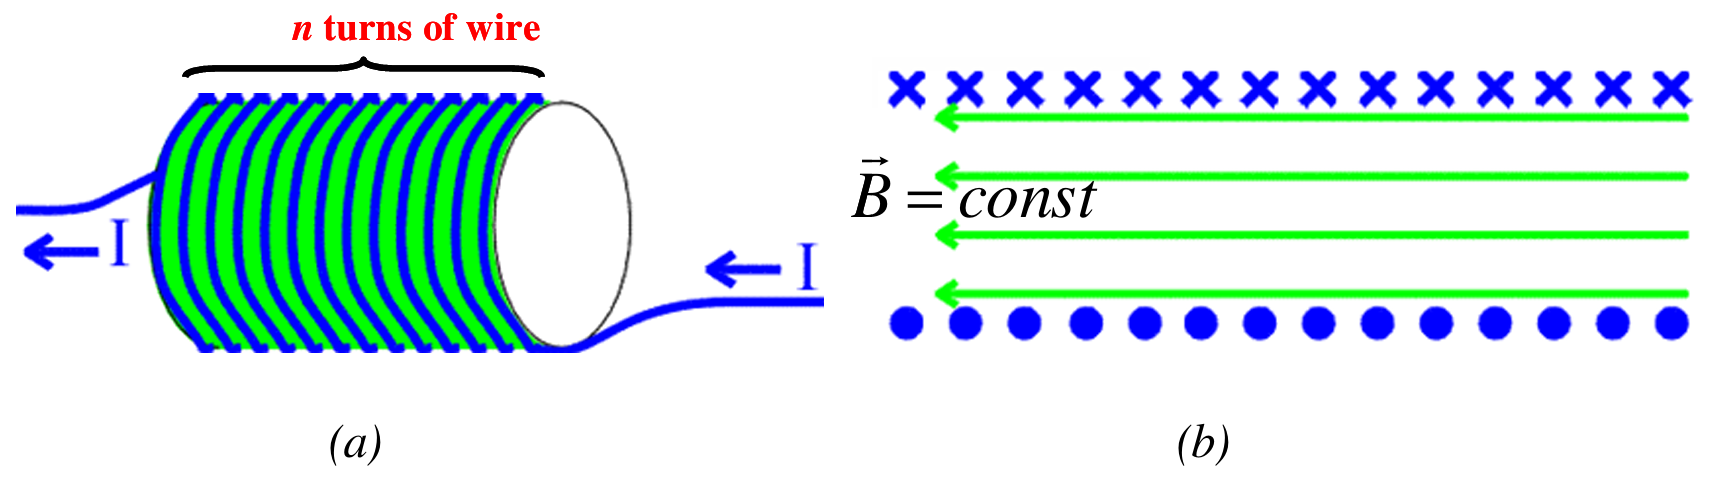
\includegraphics[width=0.85\textwidth]{Fig2}
		\captionof{figure}{\textit{ Typical solenoid (a) and magnetic field lines produced by the currents in it (b)  }}
	\end{center}
	\noindent
	Exact calculations for a long, closely wound solenoid, half of these field lines emerge from the ends and half "leak out" through the windings between the center and the ends. Because all turns carry the same current $I$. then, the total $B$ field at every point is the vector sum of the fields caused by the individual turns. For a unit of length of solenoid $ds$ with $n$ turns (Fig.3), we have
	\begin{equation}
		dB = \dfrac{\mu_0 \mu_r}{2}\dfrac{R^2}{r^3}\cdot I \cdot n \cdot ds
	\end{equation}
	\noindent
	Let point A in Fig. 3 be the reference point, with the positive direction chosen from left to right. It can be seen that $s = -R\cdot \cot \gamma$ $\left(\text{or }ds = R \cdot \dfrac{d\gamma}{\sin^2 \gamma}\right)$, and $\sin \gamma = \dfrac{R}{r}$. Hence, we obtain
	\begin{equation}
		dB = \dfrac{\mu_0 \mu_r}{2}\cdot I \cdot n \cdot \sin \gamma d\gamma
	\end{equation}
	\begin{center}
		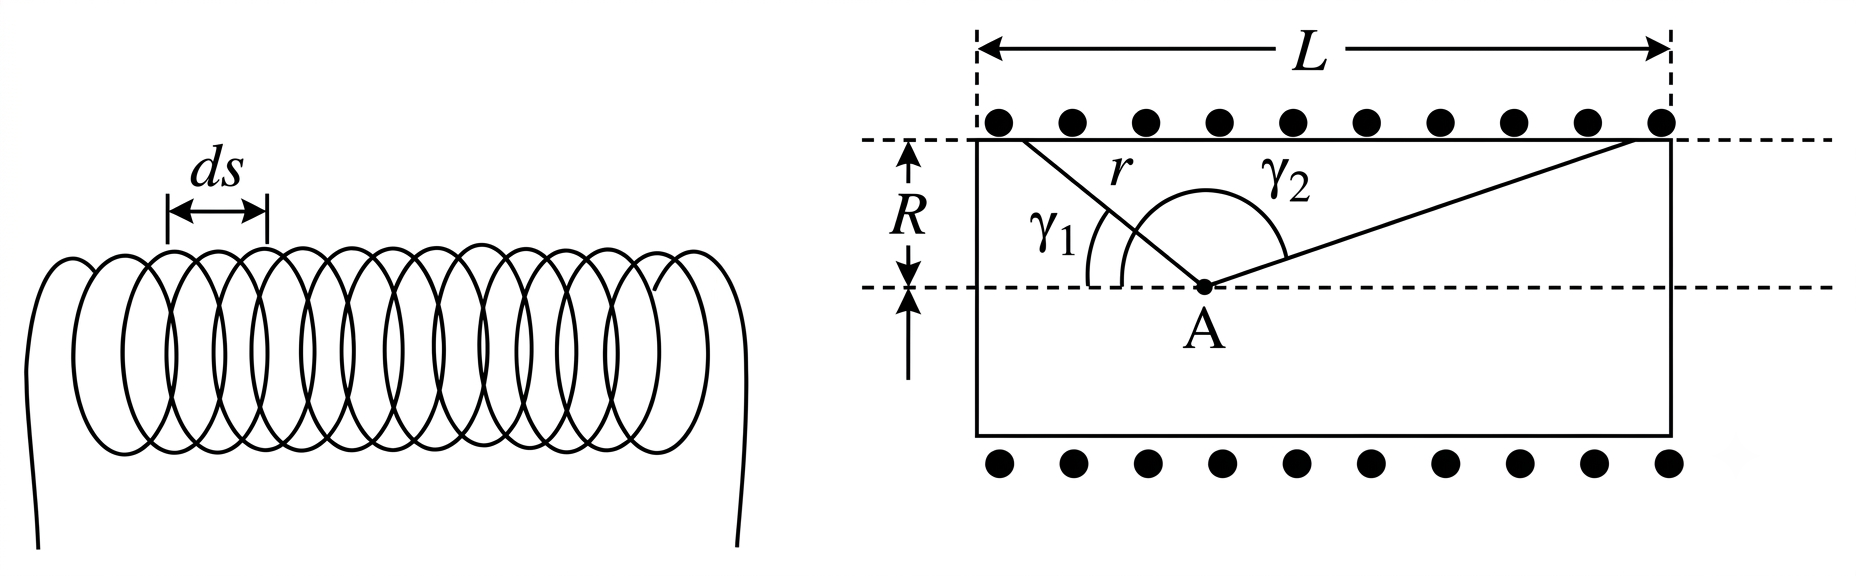
\includegraphics[width=0.85\textwidth]{Fig3}
		\captionof{figure}{\textit{The way to calculate the magnetic field at a point inside a finite solenoid}}
	\end{center}
	
	\noindent
	Using Ampere's law, the magnetic field B produced by a finite solenoid with length L at A as shown in Fig.3 would be
	\begin{equation}
		B = \frac{\mu_0\mu_r}{2} \cdot I \cdot n_0 \int\limits_{\gamma_1}^{\gamma_2} \sin\gamma \, d\gamma = \frac{\mu_0\mu_r}{2} \cdot I \cdot n_0 (\cos\gamma_1 - \cos\gamma_2)
	\end{equation}
	\noindent
	where $n_0 = \dfrac{n}{L}$ is the number of turns per unit length, if the solenoid has $n$ wire turns.
	
	\noindent
	For an infinitely long solenoid ($\gamma_1 = 0$, $\gamma_2 = \pi$), the magnetic field becomes:
	\begin{equation}
		B = \mu_0 \mu_r I n_0
	\end{equation}
	\noindent
	It can be seen that magnetic field produced by a finite coil is smaller than that by an infinite one. Clearly, the magnetic field inside is homogeneous and its strength does not depend on the distance from the axis. This last result, which holds strictly true only near the centre of the solenoid where the field lines are parallel to its length, is the most important.
	
	\section*{3. EXPERIMENTAL PROCEDURE}
	
	\subsection*{3.1. Preparation of Measurement}
	Using wires to connect the solenoid, rheostat and ammeter together in series circuit as 
	shown in Fig. 4. In this circumstance, the current provided by an AC power supply, flows 
	through the rheostat then the solenoid. The rheostat is used to monitor the magnitude of current, which is read out with an ammeter. The axial magnetic-induction probe inside solenoid 
	measures the component of the magnetic field along the solenoid symmetry axis. The axial 
	probe can be moved easily along the solenoid. The position of the probe is determined using a 
	linear rule attached with the probe. The magnetic field is read out by the Teslameter. Check if the axial probe had connected with Teslameter. 
	\begin{center}
		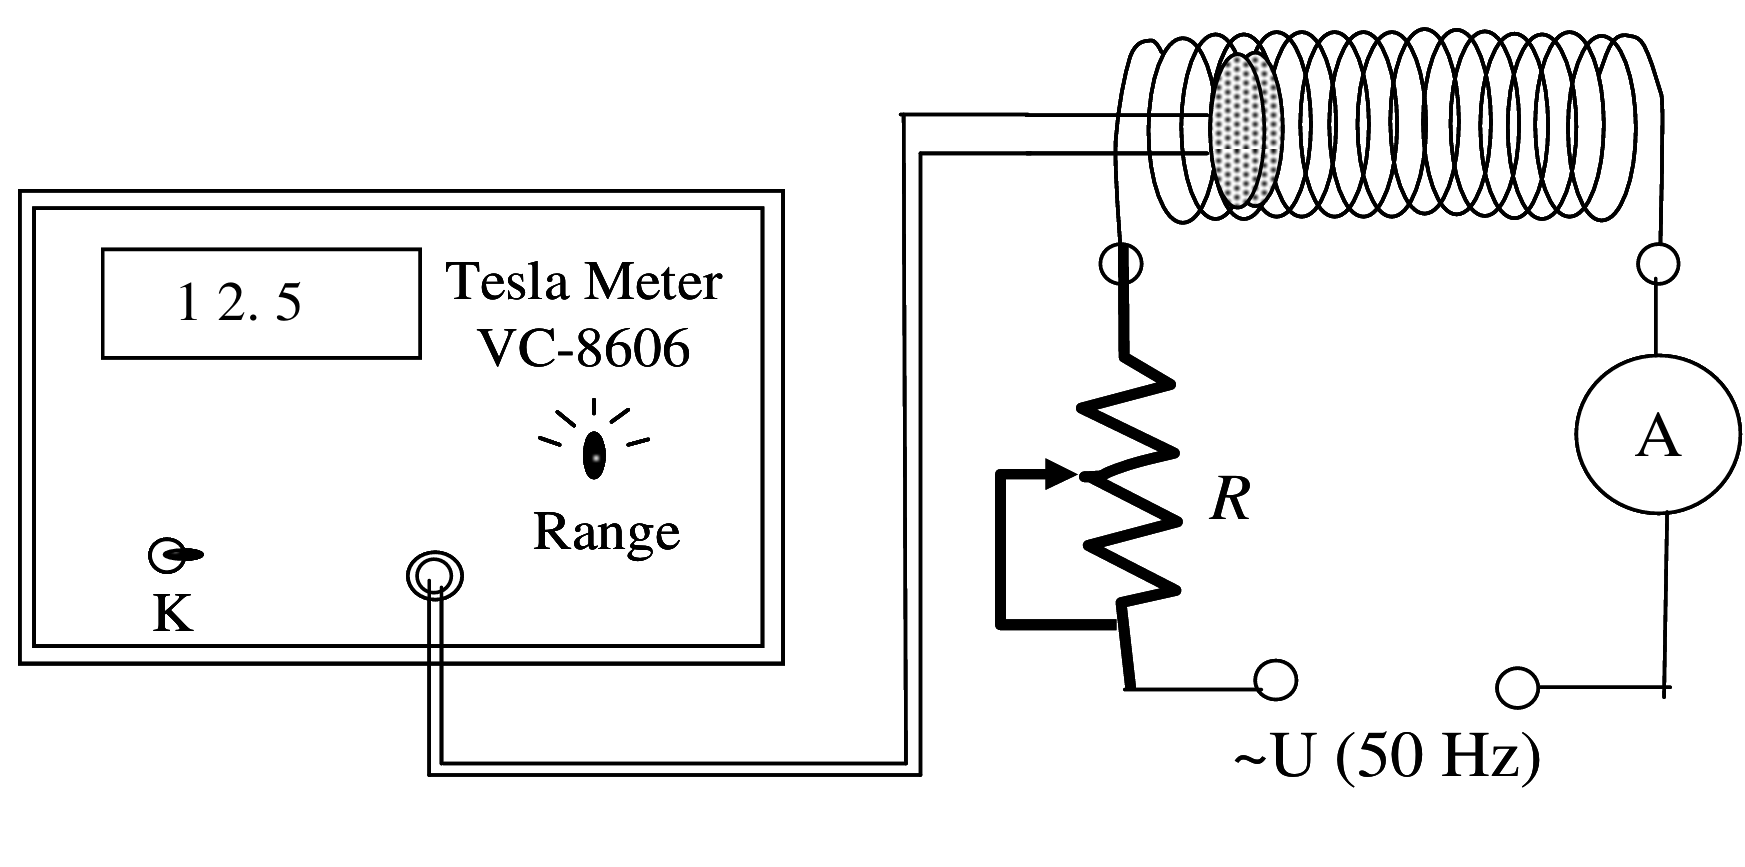
\includegraphics[width=0.5\textwidth]{Fig4}
		\captionof{figure}{\textit{Layout of measurement circuit}}
	\end{center}
	
	
	\subsection*{3.2. Measurement Sequence}
	\subsubsection*{3.2.1. Investigation of magnetic field along the axis - $B(x)$}
	\begin{enumerate}[leftmargin=1.5em]
		\item Place the axial probe so that one end of the solenoid corresponds to position $0$ on the linear rule. Set the power supply voltage to $3\,\text{V}$, turn on the power supply and Teslameter, and record the initial current and magnetic field $B(0)$.
		\item Slowly pull out the probe in increments of $1\,\text{cm}$ up to $30\,\text{cm}$, recording the magnetic field $B(x)$ at each position in Table 1.
	\end{enumerate}
	
	\subsubsection*{3.2.2. Relationship between magnetic field and current - $B(I)$}
	\begin{enumerate}[leftmargin=1.5em]
		\item Fix the axial probe at the center of the coil ($x = 15\,\text{cm}$).
		\item Set the power supply output voltage to $3\,\text{V}$, $6\,\text{V}$, $9\,\text{V}$, and $12\,\text{V}$ successively, recording the current and magnetic field $B(x)$ in Table 2.
	\end{enumerate}
	
	\subsubsection*{3.2.3. Comparison of experimental and theoretical magnetic field}
	\begin{enumerate}[leftmargin=1.5em]
		\item Adjust the rheostat so the ammeter reads $0.4\,\text{A}$ and keep it fixed.
		\item Measure the magnetic field at positions $x = 0\,\text{cm}$, $15\,\text{cm}$, and $30\,\text{cm}$, recording the results in Table 3.
	\end{enumerate}
	
	\section*{4. EXPERIMENTAL RESULTS}
	
	\subsection*{4.1. Investigation of the magnetic field at the positions along the axis of solenoid}
	
	\begin{table}[H]
		\centering
		\caption{Measurement of magnetic field $B(x)$ along the solenoid axis with $I = 0.19\text{A}$}
		\begin{tabular}{|>{\centering\arraybackslash}m{1.5cm}|>{\centering\arraybackslash}m{3.5cm}|>{\centering\arraybackslash}m{1.5cm}|>{\centering\arraybackslash}m{3.5cm}|}
			\hline
			\textbf{$x$ (cm)} & \textbf{$B(x)$ (mT)} & \textbf{$x$ (cm)} & \textbf{$B(x)$ (mT)} \rule[-0.2cm]{0pt}{0.6cm} \\
			\hline
			0 & 0.42 & 16 & 0.89 \rule[-0.25cm]{0pt}{0.7cm} \\ \hline
			1 & 0.65 & 17 & 0.89 \rule[-0.25cm]{0pt}{0.7cm} \\ \hline
			2 & 0.76 & 18 & 0.89 \rule[-0.25cm]{0pt}{0.7cm} \\ \hline
			3 & 0.81 & 19 & 0.88 \rule[-0.25cm]{0pt}{0.7cm} \\ \hline
			4 & 0.84 & 20 & 0.88 \rule[-0.25cm]{0pt}{0.7cm} \\ \hline
			5 & 0.85 & 21 & 0.88 \rule[-0.25cm]{0pt}{0.7cm} \\ \hline
			6 & 0.88 & 22 & 0.88 \rule[-0.25cm]{0pt}{0.7cm} \\ \hline
			7 & 0.88 & 23 & 0.87 \rule[-0.25cm]{0pt}{0.7cm} \\ \hline
			8 & 0.88 & 24 & 0.87 \rule[-0.25cm]{0pt}{0.7cm} \\ \hline
			9 & 0.88 & 25 & 0.86 \rule[-0.25cm]{0pt}{0.7cm} \\ \hline
			10 & 0.88 & 26 & 0.85 \rule[-0.25cm]{0pt}{0.7cm} \\ \hline
			11 & 0.88 & 27 & 0.82 \rule[-0.25cm]{0pt}{0.7cm} \\ \hline
			12 & 0.89 & 28 & 0.77 \rule[-0.25cm]{0pt}{0.7cm} \\ \hline
			13 & 0.89 & 29 & 0.68 \rule[-0.25cm]{0pt}{0.7cm} \\ \hline
			14 & 0.89 & 30 & 0.47 \rule[-0.25cm]{0pt}{0.7cm} \\ \hline
			15 & 0.89 & \multicolumn{2}{c|}{---}\rule[-0.25cm]{0pt}{0.7cm} \\ \hline
		\end{tabular}
	\end{table}
	\begin{figure}[H]
		\centering
		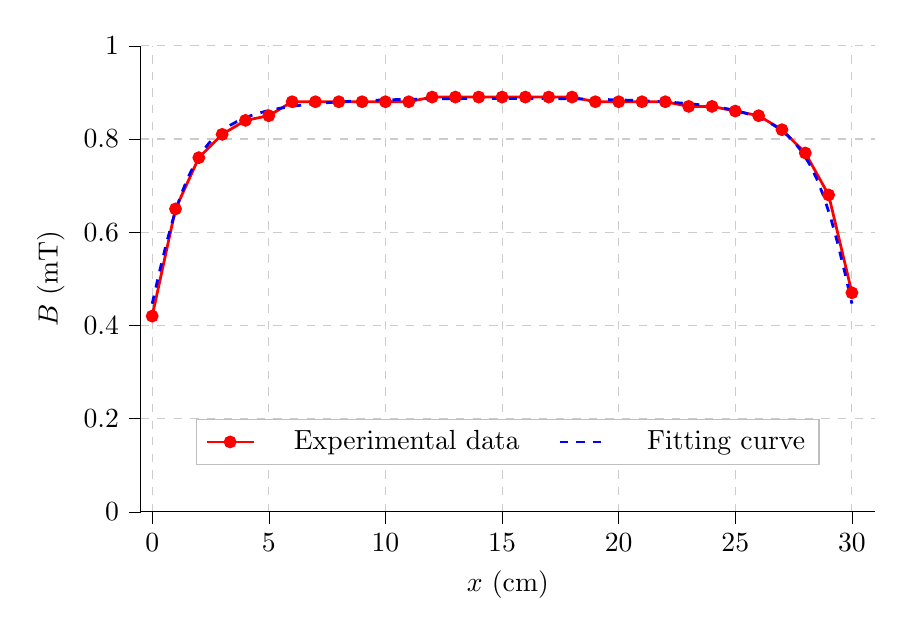
\begin{tikzpicture}
			\begin{axis}[
				width=0.9\textwidth,
				height=7.5cm,
				xlabel={$x$ (cm)},
				ylabel={$B$ (mT)},
				xmin=-0.5, xmax=31,
				ymin=0.0, ymax=1.0,
				xtick={0,5,10,15,20,25,30},
				ytick={0.0,0.2,0.4,0.6,0.8,1.0},
				yticklabel style={/pgf/number format/fixed, /pgf/number format/precision=1},
				grid=major,
				grid style={dashed, gray!40},
				axis lines=left,
				axis line style={-},
				tick align=outside,
				tick style={black},
				legend columns=-1,
				legend style={
					at={(0.5,0.2)},
					anchor=north,
					column sep=12pt,
					draw=gray!50,
				},
				]
				\addplot[
				color=red,
				line width=1pt,
				mark=*,
				mark size=1.8pt,
				] coordinates {
					(0, 0.42)  (1, 0.65)  (2, 0.76)  (3, 0.81)  (4, 0.84)  (5, 0.85)
					(6, 0.88)  (7, 0.88)  (8, 0.88)  (9, 0.88)  (10, 0.88) (11, 0.88)
					(12, 0.89) (13, 0.89) (14, 0.89) (15, 0.89) (16, 0.89) (17, 0.89)
					(18, 0.89) (19, 0.88) (20, 0.88) (21, 0.88) (22, 0.88) (23, 0.87)
					(24, 0.87) (25, 0.86) (26, 0.85) (27, 0.82) (28, 0.77) (29, 0.68)
					(30, 0.47)
				};
				\addplot[
				color=blue,
				dashed,
				line width=1pt,
				domain=0:30,
				samples=100,
				] {0.895 * 0.5 * (x/sqrt(2.015^2 + x^2) + (30 - x)/sqrt(2.015^2 + (30 - x)^2))};
				\addlegendentry{Experimental data}
				\addlegendentry{Fitting curve}
			\end{axis}
		\end{tikzpicture}
		\caption{Distribution of magnetic field $B(x)$ along the solenoid axis}
	\end{figure}
	
	\subsection*{4.2. Measurement of the relationship between the magnetic field and the current through the solenoid}
	\begin{table}[H]
		\centering
		\caption{Measurement of magnetic field $B$ versus voltage $U$ and current $I$}
		\begin{tabular}{|>{\centering\arraybackslash}m{2.5cm}|>{\centering\arraybackslash}m{3.5cm}|>{\centering\arraybackslash}m{4.5cm}|}
			\hline
			\textbf{Trial} & \textbf{Current $I$ (A)} & \textbf{Magnetic Field $B$ (mT)} \rule[-0.2cm]{0pt}{0.6cm} \\
			\hline
			1 & 0.1 & 0.53 \rule[-0.25cm]{0pt}{0.7cm} \\ \hline
			2 & 0.2 & 0.93 \rule[-0.25cm]{0pt}{0.7cm} \\ \hline
			3 & 0.3 & 1.34 \rule[-0.25cm]{0pt}{0.7cm} \\ \hline
			4 & 0.4 & 1.75 \rule[-0.25cm]{0pt}{0.7cm} \\ \hline
			5 & 0.5 & 2.21 \rule[-0.25cm]{0pt}{0.7cm} \\ \hline
			6 & 0.6 & 2.65 \rule[-0.25cm]{0pt}{0.7cm} \\ \hline
		\end{tabular}
	\end{table}
	\begin{figure}[H]
		\centering
		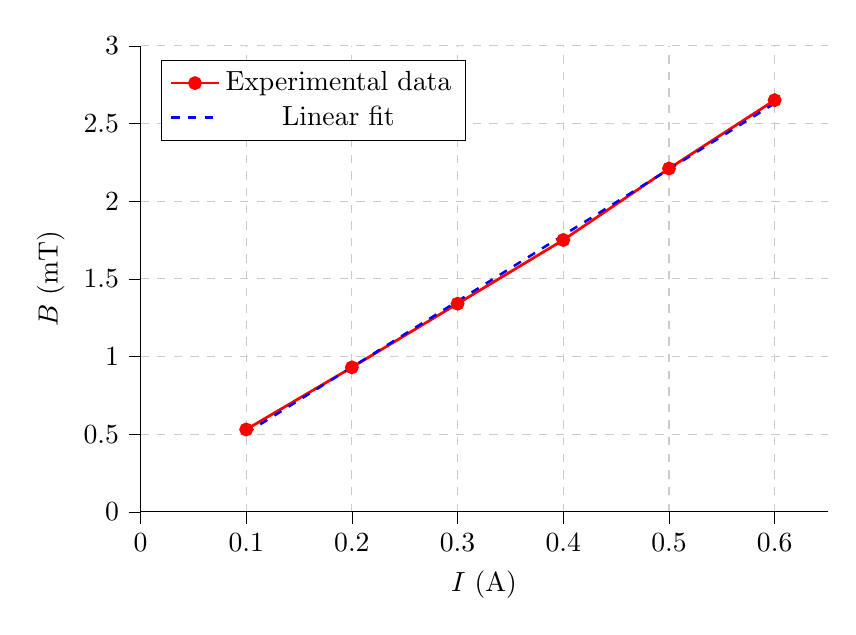
\begin{tikzpicture}
			\begin{axis}[
				width=0.85\textwidth,
				height=7.5cm,
				xlabel={$I$ (A)},
				ylabel={$B$ (mT)},
				xmin=0.0, xmax=0.65,
				ymin=0.0, ymax=3.0,
				xtick={0.0,0.1,0.2,0.3,0.4,0.5,0.6},
				ytick={0.0,0.5,1.0,1.5,2.0,2.5,3.0},
				xticklabel style={/pgf/number format/fixed, /pgf/number format/precision=1},
				yticklabel style={/pgf/number format/fixed, /pgf/number format/precision=1},
				grid=major,
				grid style={dashed, gray!40},
				axis lines=left,
				axis line style={-},
				tick align=outside,
				tick style={black},
				legend pos=north west,
				]
				% Dữ liệu thực nghiệm
				\addplot[
				color=red,
				line width=1pt,
				mark=*,
				mark size=2pt,
				] coordinates {
					(0.1, 0.53)
					(0.2, 0.93)
					(0.3, 1.34)
					(0.4, 1.75)
					(0.5, 2.21)
					(0.6, 2.65)
				};
				\addlegendentry{Experimental data}
				
				% Đường fit tuyến tính (tùy chọn - xóa 4 dòng dưới nếu chỉ muốn vẽ đường nối điểm đo)
				\addplot[
				color=blue,
				dashed,
				line width=0.9pt,
				domain=0.1:0.6,
				] {4.2457*x + 0.0823};
				\addlegendentry{Linear fit}
			\end{axis}
		\end{tikzpicture}
		\caption{Dependence of magnetic field $B$ on current $I$}
	\end{figure}
	
	\subsection*{4.3. Comparison of experimental and theoretical magnetic field }
	
	\noindent
	Two angles $\gamma_1, \gamma_2$ from Eq.(4) are determined by
	\begin{center}
		\vspace{-0.8cm}
		\begin{displaymath}
			\begin{aligned}
				&\cos \gamma_1 = \dfrac{x}{\sqrt{R^2 + x^2}} \\
				&\cos \gamma_2 = \dfrac{-\left(L - x\right)}{\sqrt{R^2 + (L - x)^2}} 
			\end{aligned}
		\end{displaymath}
	\end{center}
	Since an alternating current (AC) source is used, the ammeter measures the root-mean-square current $I = 0.4\text{ A}$, whereas the teslameter records the peak magnetic field amplitude $B_0$. Therefore, the peak current $I_0 = I\sqrt{2}$ is substituted into Eq.(4) to evaluate the theoretical peak magnetic field
	\begin{equation*}
		B_{\text{theo}} = \frac{\mu_0 \mu_r I_0 n_0}{2} (\cos\gamma_1 - \cos\gamma_2) = \frac{\mu_0 \mu_r I\sqrt{2}\, n_0}{2} (\cos\gamma_1 - \cos\gamma_2)
	\end{equation*}
	\noindent
	 With the solenoid having the number of wire turns $n = 750$, length $L = 300\text{mm} = 30\text{cm}$, diameter of the cross-section $D = 40.3\text{mm}$, $\mu_r = 1$ (since the environment is air), we yield
	\begin{center}
		\fbox{%
			\begin{minipage}{0.8\textwidth}
				\vspace{-0.4cm}
				\centering
				\begin{displaymath}
					\begin{aligned}
						&x = 0\text{ cm} &\implies B_\text{theo} \approx 0.89\text{ mT} \\
						&x = 15\text{ cm} &\implies B_\text{theo} \approx 1.76\text{ mT} \\
						&x = 30\text{ cm} &\implies B_\text{theo} \approx 0.89\text{ mT}
					\end{aligned}
				\end{displaymath}
			\end{minipage}%
		}
	\end{center}
	\begin{table}[H]
		\centering
		\caption{Comparison of experimental and theoretical magnetic field at $I = 0.4\,\text{A}$}
		\begin{tabular}{|>{\centering\arraybackslash}m{2.5cm}|>{\centering\arraybackslash}m{3.5cm}|>{\centering\arraybackslash}m{3.5cm}|>{\centering\arraybackslash}m{3cm}|}
			\hline
			\textbf{Position $x$ (cm)} & \textbf{$B_{\text{exp}}$ (mT)} & \textbf{$B_{\text{theo}}$ (mT)} & \textbf{Relative Error (\%)} \rule[-0.2cm]{0pt}{0.6cm} \\
			\hline
			0  & 0.85 & 0.89 & 4.13 \rule[-0.25cm]{0pt}{0.7cm} \\ \hline
			15 & 1.75 & 1.76 & 0.64 \rule[-0.25cm]{0pt}{0.7cm} \\ \hline
			30 & 0.92 & 0.89 & 3.77 \rule[-0.25cm]{0pt}{0.7cm} \\ \hline
		\end{tabular}
	\end{table}
	
	\noindent
	From Table 3, we can conclude that the measured magnetic field magnitudes are in close agreement with the theoretical values, as evidenced by the small relative errors. Minor discrepancies arise from measurement uncertainties during data collection.
	
\end{document}